% vim:ts=4:sw=4
% Copyright (c) 2014 Casper Ti. Vector
% Public domain.

\chapter{光学波段的研究}

\section{射电脉冲星导致的微引力透镜事件及脉冲星的质量测量}

脉冲星质量的测量对于限制其内部结构有至关重要的作用。大质量的脉冲星将对
物态方程提出很强的限制,而极低质量的脉冲星有助于我们区分自束缚的夸克星
和引力束缚的中子星。近几年测量的大质量脉冲星,PSRs J0348$+$0432和J1614$-$2230,
已经刷新了我们对脉冲星物态方程和内部结构的理解\supercite{Anton,Demorest,Ozel2010,Lai2011}。
%
然而目前为止,所有精确的质量测量都是针对双星系统的。测量孤立脉冲星
的质量仍然是巨大的挑战。而孤立脉冲星的质量测量有很重要的意义,因为
孤立脉冲星很可能有与双星系统中的脉冲星不同的质量分布。

微引力透镜效应是可能的测量孤立脉冲星质量的一种方法\supercite{Dai,Schwarz02,Horvath96}。
当一个致密的天体比较近地穿过我们与一个背景天体的视线方向时,有两种微引力透镜
效应可能发生。一种效应被称作photometric microlensing,这种效应被观测为背景
天体亮度的变化。对于photometric microlensing,背景天体亮度的放大倍数($A$)
与透镜天体和背景天体之间的角距离有关,关系为$A\sim 1+2/u^{4}$\supercite{mao},
其中以Einstein半径为单位的角距离被定义为$u=\theta_{\rm{sl}}/\theta_{\rm{E}}$。
对于银河系中的天体,典型的Einstein角半径的大小是约1\,mas。
%
第二种效应被称作astrometric microlensing,这种效应被观测为背景天体的光学中心
的移动($S$)。当透镜天体和背景天体的角距离($u$)大于Einstein半径($\theta_{\rm{E}}$)
时,背景天体光学中心的移动与透镜天体和背景天体的角距离的关系为$S \sim \theta_{\rm{E}}/u$\supercite{Bel}。
因此,我们可以看到astrometric microlensing的效应随透镜天体与背景天体的角距离
的衰减比photometric microlensing慢,所以astrometric microlensing事件发生的
“截面(cross-section)”更大、概率更高。但是目前的望远镜还很难做大范围的astrometic现
象的巡天。

Optical Gravitational Lensing Experiment (OGLE)~\supercite{Udalski}是一个
正在进行中的photmetric microlensing事件的巡天项目。这个项目的第三阶段(third phase,
OGLE-III)监测了银河系核球中约$3\times10^{8}$个天体\supercite{Szymanski}。
目前正在进行中的第四阶段(OGLE-IV)的天空覆盖范围比OGLE-III更大,并且现在
每年在核球和麦哲伦云(Magellanic Clouds)方向发现的微引力透镜事件数大概是
OGLE-III的四倍。在不远的将来,Large Synoptic Survey Telescope (LSST)\supercite{lsst}
将发现大量的微引力透镜事件。

目前以及可预见的将来将不会有大范围的astrometric microlensing的巡天项目。
然而如果astrometric microlensing事件可以被预测,那么我们就可以使用现有
望远镜进行某个特定天区的观测而不需要进行巡天。对于有射电辐射的脉冲星,
我们可以独立的通过射电观测确定脉冲星的天体测量参数,从而使我们可以预计
由脉冲星导致的astrometric microlensing事件的发生时间和位置。更重要的是,射电
脉冲星的距离也可以通过射电观测独立估计,于是对这样的微引力透镜事件,我们可以
直接地测量脉冲星的质量。目前,我们只发现了银河系内的一小部分射电脉冲星。
未来的射电望远镜(比如FAST\supercite{Nan}和SKA\supercite{Johnston2007})
有能力发现银河系内的大部分可观测到的射电脉冲星,并且能精确地测量大量
射电脉冲星的天体测量参数。因此我们有望预测由射电脉冲星导致的微引力透镜
事件,并以此测量脉冲星的质量。

\subsection{中子星导致的photometric microlensing事件的性质}

在这一节中,我们研究由中子星导致的photometric microlensing事件的性质。
我们考虑中子星作为透镜天体,而银河系内的天体和遥远的星系可以作为背景
天体。Tian \& Mao (2012)\supercite{Tian}研究了中子星作为透镜天体,引起
的背景星系的弱引力透镜效应,因此我们将只考虑银河系内的天体作为背景
天体。我们使用的方法主要参考了Wood \& Mao (2005)\supercite{Wood}的
工作(缩写为WM05)。我们将首先描述我们使用的中子星的空间和速度分布
模型,以及银河系内天体的模型。然后我们将给出事件概率、事件时标的分布
以及中子星导致的微引力透镜事件在银河系总的透镜事件中占的比例。

\subsubsection{中子星的分布模型}

我们假设中子星的分布是正比于射电脉冲星的分布的。在以银河系中心
(Galactic Center,GC)为中心的柱坐标系中,中子星的分布可以表示为
%
\begin{equation}
\begin{split}
\rho(R,z) & =A\left(\frac{R+R_{1}}{R_{\odot}+R_{1}}\right)^{\rm{a}}\exp\left[-b\left(\frac{R-R_{\odot}}{R_{\odot}+R_{1}}\right)\right]\\
          & \times\exp\left(-\frac{|z|}{E}\right),
\end{split}
\end{equation}
%
其中$R_{1}=0.55$\,kpc,$a=1.64$,$b=4.01$,$E=330$\,pc,太阳到银河系
中心的距离是$R_{\odot}=8.0$\,kpc。我们使用了Yusifov \& K{\"u}{\c c}{\"u}k 
(2004)\supercite{Yusifov}建议的中子星的径向分布。这样的径向分布也被
Faucher-Gigu{\`e}re \& Kaspi (2006)\supercite{Faucher}采用,并且使
我们可以直接使用Faucher-Gigu{\`e}re \& Kaspi (2006)预测的银河系中可
观测的脉冲星的数目。在$z$方向上,我们使用了Lorimer et al. (2006)\supercite{Lorimer06}
给出的分布。

银河系中总的中子星的数目现在仍然不清楚。根据最近的Keane \& Kramer (2008)\supercite{Keane}
的工作,我们调整参数$A$的数值,给出总的中子星数目为$10^9$。对于可观测的
脉冲星,根据Faucher-Gigu{\`e}re \& Kaspi (2006)\supercite{Faucher}的模拟,我们
调整参数$A$的数值,给出总的数目为120000。值得指出的是,我们使用的可观测
脉冲星的数值并没有考虑Rotating Radio Transients\supercite{McLaughlin06}。
考虑了这一类中子星后,可观测脉冲星的数目将大幅增加\supercite{Keane}。

对于中子星的速度分量,我们使用了高斯分布来模拟,高斯分布的参数是
$\sigma=290\ \rm{km\ s^{-1}}$\supercite{Faucher}。在后面我们会提到,
微引力透镜事件的时标和事件概率分别是反比和正比于透镜天体和背景天体
的相对速度的。因此,增大或者减小中子星速度分布的$\sigma$将直接地
缩放时标和事件概率。尽管Faucher-Gigu{\`e}re \& Kaspi (2006)更倾向于
指数分布,但是高斯分布同样能很好地符合观测到的射电脉冲星的速度分布\supercite{hobbs},
并且给我们提供了一个更直接的分布,简化我们的计算。在后面的分析中,
我们主要使用高斯分布模型,但是作为对比我们也使用指数模型给出了一些
结果。

\subsubsection{银河系天体的分布模型}

为了确定背景天体的性质,我们考虑了银河系的盘和银核中的天体的分布。
对于银核中的天体,我们使用了Rattenbury et al. (2007)\supercite{Rattenbury}
中给出的E2模型。我们把银核在公转半径$R_{C}=3.5$\,kpc~\supercite{Bissantz}
处截断。我们使用了银河系中心方向上观测得到的微引力透镜事件光深来归一化
我们使用的分布\supercite{Calchi,popowski}。银河系盘上的天体的分布是
研究得比较透彻的,于是我们使用了被Han \& Gould (2003)\supercite{han}
推广到整个银盘的、Zheng et al. (2001)\supercite{zheng}给出的local vertical 
density model。

我们还需要不同种类的透镜天体的模型(包括中子星和其他天体)。我们使用
了WM05中采用的透镜天体的质量函数。这是一个由两部分幂律分布组成的质量函数,
%
\begin{equation}
\frac{\rm{d}N}{\rm{d}M}=k\left(\frac{M}{M_{\rm{brk}}}\right)^{\rm{\alpha}},
\end{equation}
%
其中$M_{\rm{brk}}=0.7$\,$\rm{M_{\odot}}$。对于$M>M_{\rm{brk}}$,
$\alpha=-2.0$;对于$M\leq M_{\rm{brk}}$,$\alpha=-1.3$。

我们使用了WM05给出的银河系内天体的动力学模型。这个模型描述了透镜天体、
背景天体以及观测者的速度。透镜天体和背景天体的相对速度($\upsilon$)
是根据WM05中的方程7、8计算的。我们使用了Wang \& Smith (2011)\supercite{wang}
给出的公式15,将速度从以银心为中心的柱坐标系转换到以太阳为中心的球坐标系中。

\subsubsection{Photometric microlensing模型}

微引力透镜事件的时标是指背景天体穿过透镜天体的Einstein半径($r_{\rm{E}}$)
的时间,被定义为\supercite{Paczynski1996},
%
\begin{equation}
\label{te}
t_{\rm{E}}=\frac{r_{\rm{E}}}{\upsilon},\
r_{\rm{E}}=\sqrt{\frac{4GM}{c^{2}}\frac{D_{\rm{d}}(D_{\rm{s}}-D_{\rm{d}})}{D_{\rm{s}}}},
\end{equation}
%
其中$G$是万有引力常数,$c$是光速,$D_{\rm{s}}$是背景天体的距离,$D_{\rm{d}}$是透镜天体的距离。

微引力透镜事件的事件概率($\Gamma$)被定义为对于一个背景天体,在一定
时间内的photometric microlensing事件的数目。事件概率与背景天体的数
密度($\rho_{\rm{s}}(D_{\rm{s}})$)以及透镜天体的质量密度($\rho_{\rm{m}}(D_{\rm{d}})$)
有关。根据WM05,我们假设光学亮度大于某一个亮度$L$的背景天体的比例正
比于$L^{\beta}$,于是事件概率可以表示为
%
\begin{equation}
\label{rate}
\begin{split}
\Gamma=&\frac{4G^{1/2}}{c}\int_{0}^{\infty}\rm{d}D_{\rm{s}}D_{\rm{s}}^{2+2\beta}\rho_{\rm{s}}(D_{\rm{s}})\\
	     &\frac{\int_{0}^{D_{\rm{s}}}\rm{d}D_{\rm{d}}\rho_{\rm{m}}(D_{\rm{d}})\upsilon[D_{\rm{d}}(D_{\rm{s}}-D_{\rm{d}})/MD_{\rm{s}}]^{1/2}}{\int_{0}^{\infty}\rm{d}D_{\rm{s}}D_{\rm{s}}^{2+2\beta}\rho_{\rm{s}}(D_{\rm{s}})},
\end{split}
\end{equation}
%
其中$\upsilon$是透镜天体和背景天体的相对速度。

我们使用$\beta$来模拟多种无法在公式中解析描述的效应。为了考虑背景天体的
亮度分布(luminosity function)、光学巡天的灵敏度以及银河系的消光,我们
假设$\beta$的取值范围为$-3\leq\beta\leq-1$\supercite{kiraga}。我们也计算了
$\beta=0$的情形,对应了最大的事件概率。我们采用的方法是比较简化的,但是
这种方法被之前的研究银河系微引力透镜事件概率的工作广泛使用。考虑到
我们的工作的目的是研究中子星导致的微引力透镜事件的性质,而不是预计某个
光学巡天能发现的确切的事件数目,这种简化的方法也是可行的。尽管消光现象
会明显地影响我们的估算,但是细致地模拟银河系的消光是极为复杂的\supercite{kerins}。
由于消光现象的影响主要是背景天体的亮度分布的斜率,我们是可以通过不同
的$\beta$的选择来模拟的,也就是说越小的$\beta$反应了越强的消光。
我们既考虑了银核中的背景天体,也考虑了在银盘上的背景天体。由于银盘上的
背景天体的距离可以趋近于零,这导致当$-3\leq\beta\leq-1$时我们会
计算得到非物理的趋近于零的事件概率。因此在计算中,对于距离在4.5\,kpc以
内的银盘上的天体,我们取$\beta=0$。

为了计算事件概率和平均时标,我们使用了adaptive Monte Carlo integration
的算法,并且调用了GNU Scientific Library\footnote{\url{http://www.gnu.org/software/gsl/}}。
为了提高计算的精度,我们在计算多维积分时使用的Monte Carlo模拟的采样数为$10^7$。

\subsubsection{事件概率}

我们给出的最大的($\beta = 0$)由中子星导致的全天事件概率为
$4.2\times10^{-7}$\,$\rm{yr^{-1}}$。在银心和Baade's window(BW)\footnote{$(l,b)=(1.16^{\circ},-2.75^{\circ})$, $l$和$b$是银经和银纬。} 
方向,最大事件概率分别是$6.7\times10^{-7}$\,$\rm{yr^{-1}}$
和$3.6\times10^{-7}$\,$\rm{yr^{-1}}$。取$\beta=-1,-2,-3$,全天
的事件概率分别是$1.3\times10^{-7}$\,$\rm{yr^{-1}}$、
$7.5\times10^{-8}$\,$\rm{yr^{-1}}$和$7.4\times10^{-8}$\,$\rm{yr^{-1}}$。
在表\ref{eventRate}中,我们给出了由120000颗可观测的射电脉冲星
导致的全天事件概率、对于$\mid b\mid<5^{\circ}$和$\mid
b\mid>5^{\circ}$ 以及银心和BW方向的事件概率。由于我们假设射电脉冲星
的分布和中子星的分布除了归一化因子以外是完全相同的,所以由可观测射
电脉冲星导致的事件概率与由中子星导致的事件概率有简单的关系,即可观
测射电脉冲星导致的事件概率比中子星导致的事件概率小$10^9/\left(1.2\times10^5\right)$倍。
使用中子星速度分布的指数模型,我们得到由可观测脉冲星导致的全天事件概率
是$4.2\times10^{-11}$\,$\rm{yr^{-1}}$ ($\beta=0$),作为对比,使用
高斯模型得到的结果是$5.0\times10^{-11}$\,$\rm{yr^{-1}}$。

\begin{table}
\begin{center}
\caption{由可观测射电脉冲星导致的事件概率,单位是$10^{-11}$\,$\rm{yr^{-1}}$。
由中子星导致的事件概率是表中的数值乘以$10^9/\left(1.2\times10^5\right)$。}
\label{eventRate}
\begin{tabular}{lccccc}
\hline
    $\beta$    &      All-sky  &   $\mid b\mid<5^{\circ}$  & $\mid b\mid>5^{\circ}$  & GC  &  BW        \\
%               &    \multicolumn{5}{c}{($\times10^{-11}\ \rm{yr^{-1}}$)}                                \\
\hline
      0        &      5.0      &    5.7    &  1.3  &  8.0 & 4.4   \\
      -1       &      1.5      &    2.0    &  0.5  &  5.5 & 2.8   \\
      -2       &      0.9      &    1.2    &  0.4  &  2.0 & 1.4   \\
      -3       &      0.9      &    1.2    &  0.4  &  1.9 & 1.3   \\
\hline
\end{tabular}
\end{center}
\end{table}
%
%%%%%%%%%%%%%%%%%%%%%%%%%%%%%%%%%%%%%%%%%
\begin{figure}
\begin{center}
\includegraphics[width=4 in,trim=0 0 0 3cm]{map_event_ns.eps}
\caption{在银河系中心区域,由中子星导致的微引力透镜事件概率的等值图。
实线代表$\beta=-1$的结果,彩色区域代表$\beta=-2$的结果。OGLE-III的监测区域
用菱形表示。等值图采用对数取值的,$\log(\Gamma/10^{-8}$\,$\rm{yr^{-1}})$。}
\label{map_event}
\end{center}
\end{figure}
%%%%%%%%%%%%%%%%%%%%%%%%%%%%%%%%%%%%%%%%%%
%

在图\ref{map_event}中,我们给出了在银河系中心区域的由中子星导致的微引力
透镜事件的概率。等值图采用对数取值,$\log(\Gamma/10^{-8}$\,$\rm{yr^{-1}})$。
我们给出了两组结果,实线代表$\beta=-1$,彩色区域代表$\beta=-2$。
正如我们期待的,在银盘上的事件概率比较高,随着银纬的升高事件概率下降。
随着$\beta$从$-1$变到$-2$,事件概率的分布变得更扁更平,与高银纬的区域对比,
事件概率在银盘上随着银经的升高下降得更快。

微引力透镜事件的概率随着$\beta$的减小而下降,并且事件概率的分布变平是因为:
\begin{itemize}
\item $\beta$的减小意味着遥远的背景天体对事件概率的贡献减小了。因此事件概率
随着$\beta$的减小而下降。
\item 在银心方向,天体的密度比银盘上高。因此,$\beta$的减小对银心方向的影响
更大,银心方向的事件概率随着$\beta$的减小下降更快。
\item 在银河系核心区域,天体的速度弥散更大。因此$\beta$的减小使在银河系
中心方向,高速运动的背景天体的贡献减小。
\item 在银心后面的银盘上的天体绕银心运动的速度方向是与观测者和近距离的
透镜天体的速度方向相反的,于是透镜天体和背景天体的相对运动速度更快,对事件
概率的贡献也更大。$\beta$的减小意味着这部分遥远背景天体的贡献显著下降。
\end{itemize}

在图\ref{map_event}中,OGLE-III的监测区域\footnote{数据来自\url{http://ogle.astrouw.edu.pl/}}使
用菱形表示出。对于$340\times10^6$颗背景天体\supercite{Szymanski},并且
取$\beta=-1$,我们预计OGLE-III每年可以发现50个由中子星导致的微引力透镜事件,
同时我们有6\%的机会在九年的巡天期间发现一个由可观测射电脉冲星导致的事件。
目前正在进行中的OGLE-IV从2010年开始,覆盖了比OGLE-III大得多的天区,每年
发现四倍于OLGE-III的微引力透镜事件。因此,我们预计OGLE-IV每年将探测到
约200个由中子星导致的事件,并且在2020年之前有23\%的机会发现一个由可观测
射电脉冲星导致的微引力透镜事件。对于未来的更深、天区更广的光学巡天,我们
很有希望发现由可观测射电脉冲星导致的微引力透镜事件。比如,LSST预计将
监测$\sim10^{10}$颗银河系中的天体\supercite{ivez12a},取$\beta=-1$我们
估计每年将会发现约1000个由中子星导致的微引力透镜事件,以及约2个由可观测
射电脉冲星导致的事件。

值得指出的是,我们的计算很可能低估了photometric microlensing的事件概率。
我们在计算中使用Einstein半径作为引力透镜事件发生的截面,对应的背景天体亮度的
变化是约0.32\,mag。然而,在实际观测中我们有可能可以探测
到比这个更微弱的背景天体亮度的变化。假设我们可以观测到的背景天体的亮度
变化为0.1\,mag,那么事件概率将增大70\%。另外,实际的背景天体的数目有可能
因为不可区分的多个天体的叠加而被低估了\supercite{Smith07}。
  
\subsubsection{事件时标的分布}

通过将Monte Carlo integration的参数空间限制在某个特定的事件时标范围之内,
我们可以得到由中子星导致的微引力透镜事件的概率与时标的关系。我们的
结果展示在图\ref{timescale}中,我们取$\beta=-1$。全天平均事件概率
的时标的分布用实线表示。在银心和BW方向的事件概率的时标分布分别用点线和
虚线给出。我们指出,时标的分布在长时标和短时标上的渐进形式在WM05中已经
给出,我们的结果与渐进形式是符合的。我们发现,由中子星导致的微引力透镜
事件的时标分布都在约12天左右达到最大值。对于全天的平均事件概率以及在
银心和BW方向上的事件概率,平均时标分别是$\sim19.7$、$19.3$和$19.4$天。
作为对比,我们在图\ref{timescale}中也给出了WM05对中子星导致的事件
的时标的预测,其对应的平均时标是约47.3天。我们的结果说明,考虑了
中子星的空间和速度分布后,由中子星导致的事件的时标比之前工作的预计
短,这主要是因为中子星有比较高的速度。使用指数速度模型,我们得到
的全天平均事件概率的平均时标是约23.7天。

在图\ref{timescale_beta}中,我们展示了调整$\beta$对于银心方向的由中子星
导致的事件的时标分布的影响。当$\beta$从$-1$减小到$-2$,事件概率时标分布的变化
远比其他的$\beta$值大,这是因为当$\beta=-2$,根据式子\ref{rate}中
的$D_{\rm{s}}^{2+2\beta}$项,背景天体的密度开始随着距离的增加而减小。
对于时标比平均时标短的事件,改变$\beta$对事件概率的影响非常小。而对于
长时标的事件,改变$\beta$有明显的影响,随着$\beta$的减小事件概率降低。
然而,平均时标随着$\beta$的变化并不剧烈。取$\beta$在0到$-3$,平均时标
分别是19.3、17.9、13.5和13.2天。我们得到的平均时标的变化很难直观地
从物理图像上理解,因为随着$\beta$减小遥远的背景天体的贡献减小,我们预期
平均的透镜天体和背景天体的相对速度会减小,短时标的事件的概率会减小。
为了理解我们的结果,我们分别计算了平均的Einstein半径和透镜天体和背景天体
的相对速度。我们发现,随着$\beta$的减小,平均的Einstein半径和透镜天体
和背景天体的相对速度都减小,但是Einstein半径减小得更快。这就解释了随
着$\beta$减小平均时标减小。

%%%%%%%%%%%%%%%%%%%%%%%%%%%%%%%%%%%%%%%%%
\begin{figure}
\begin{center}
 % 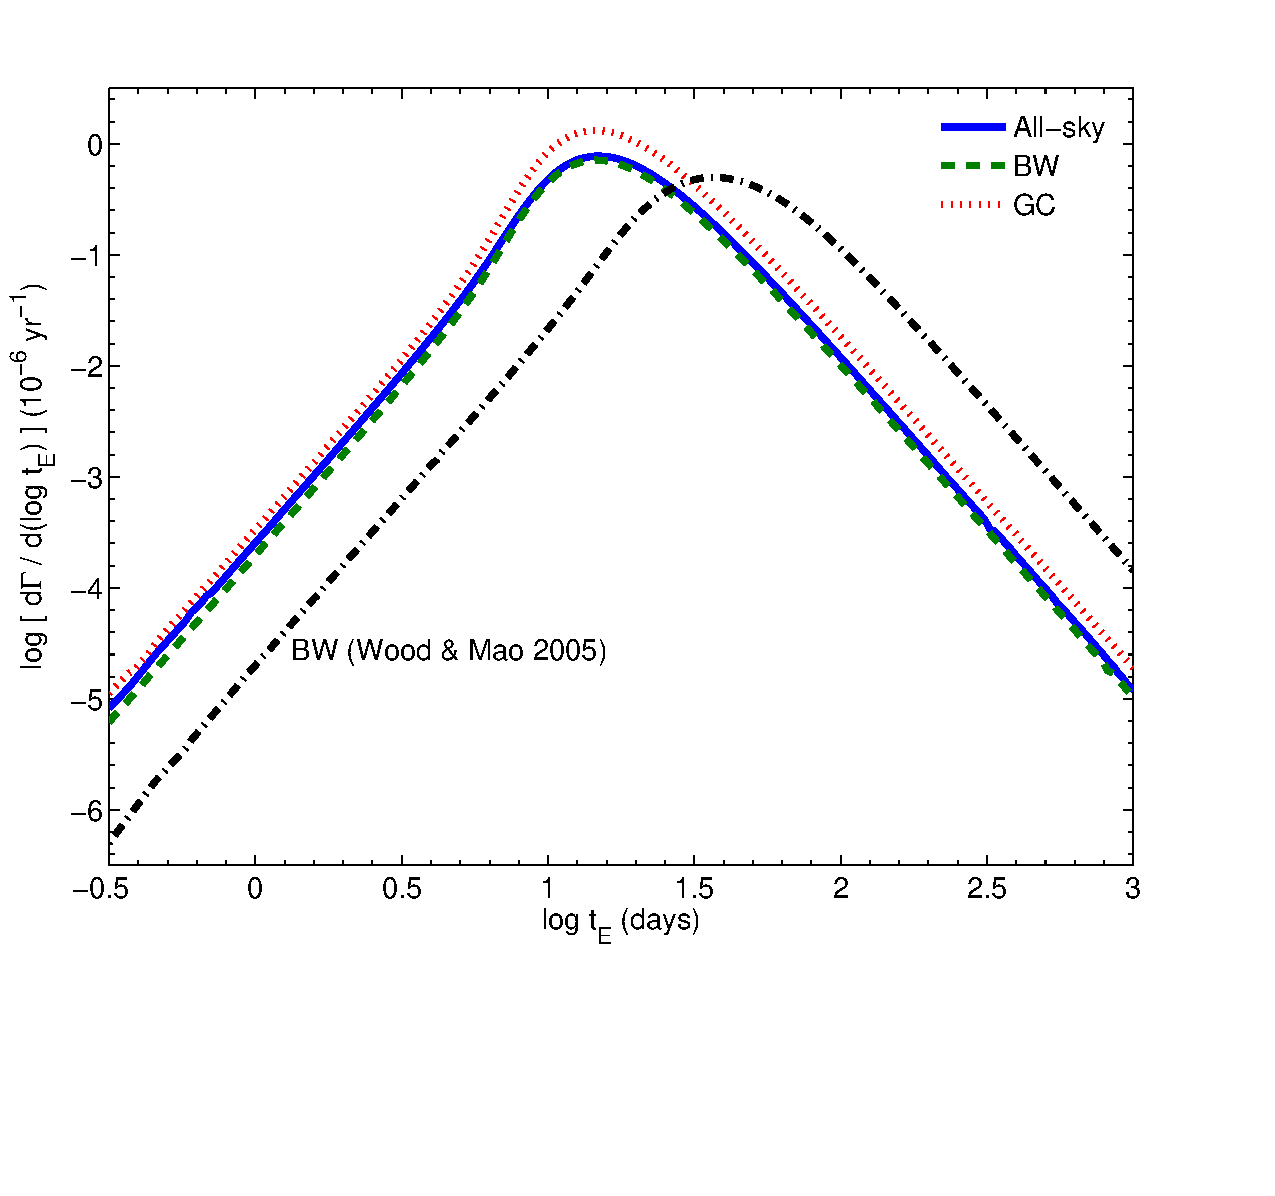
\includegraphics[width=4 in]{timescale.eps}
  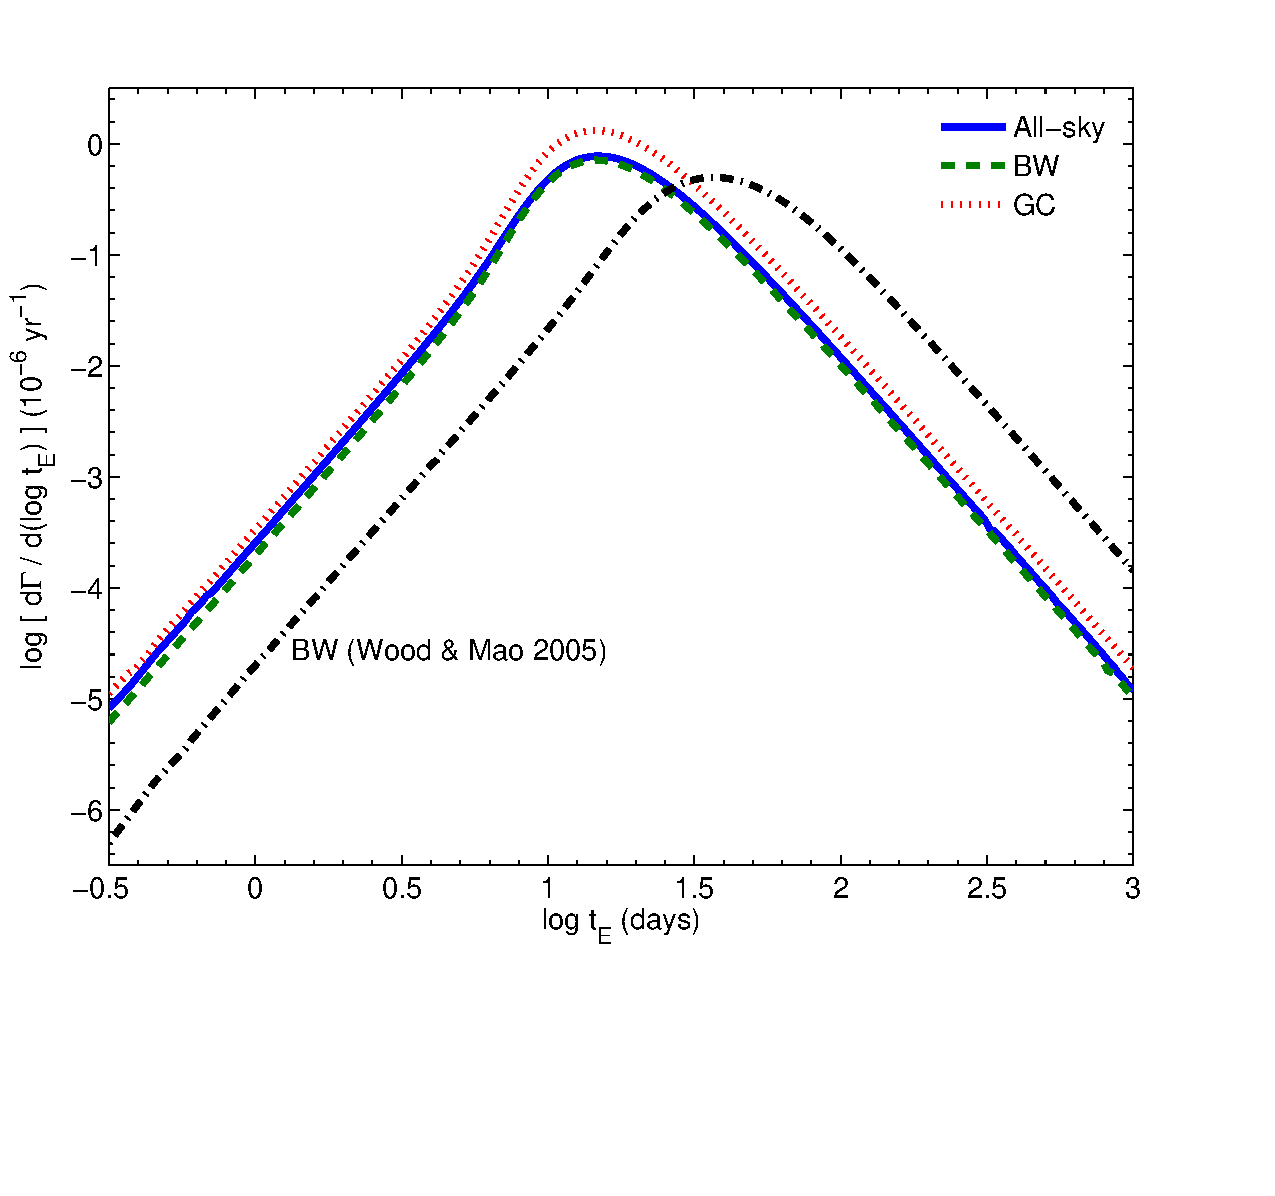
\includegraphics[width=4 in,trim=0 0 0 3cm]{timescale.eps}
\caption{中子星导致的微引力透镜事件的概率随时标的分布。实线、点线和虚线分别
对应全天事件概率、银心和BW方向的事件概率。作为对比,我们也给出了WM05的模型
对于中子星导致的事件的预言。}
\label{timescale}
\end{center}
\end{figure}
%%%%%%%%%%%%%%%%%%%%%%%%%%%%%%%%%%%%%%%%%

%
%%%%%%%%%%%%%%%%%%%%%%%%%%%%%%%%%%%%%%%%%
\begin{figure}
\begin{center}
  %
  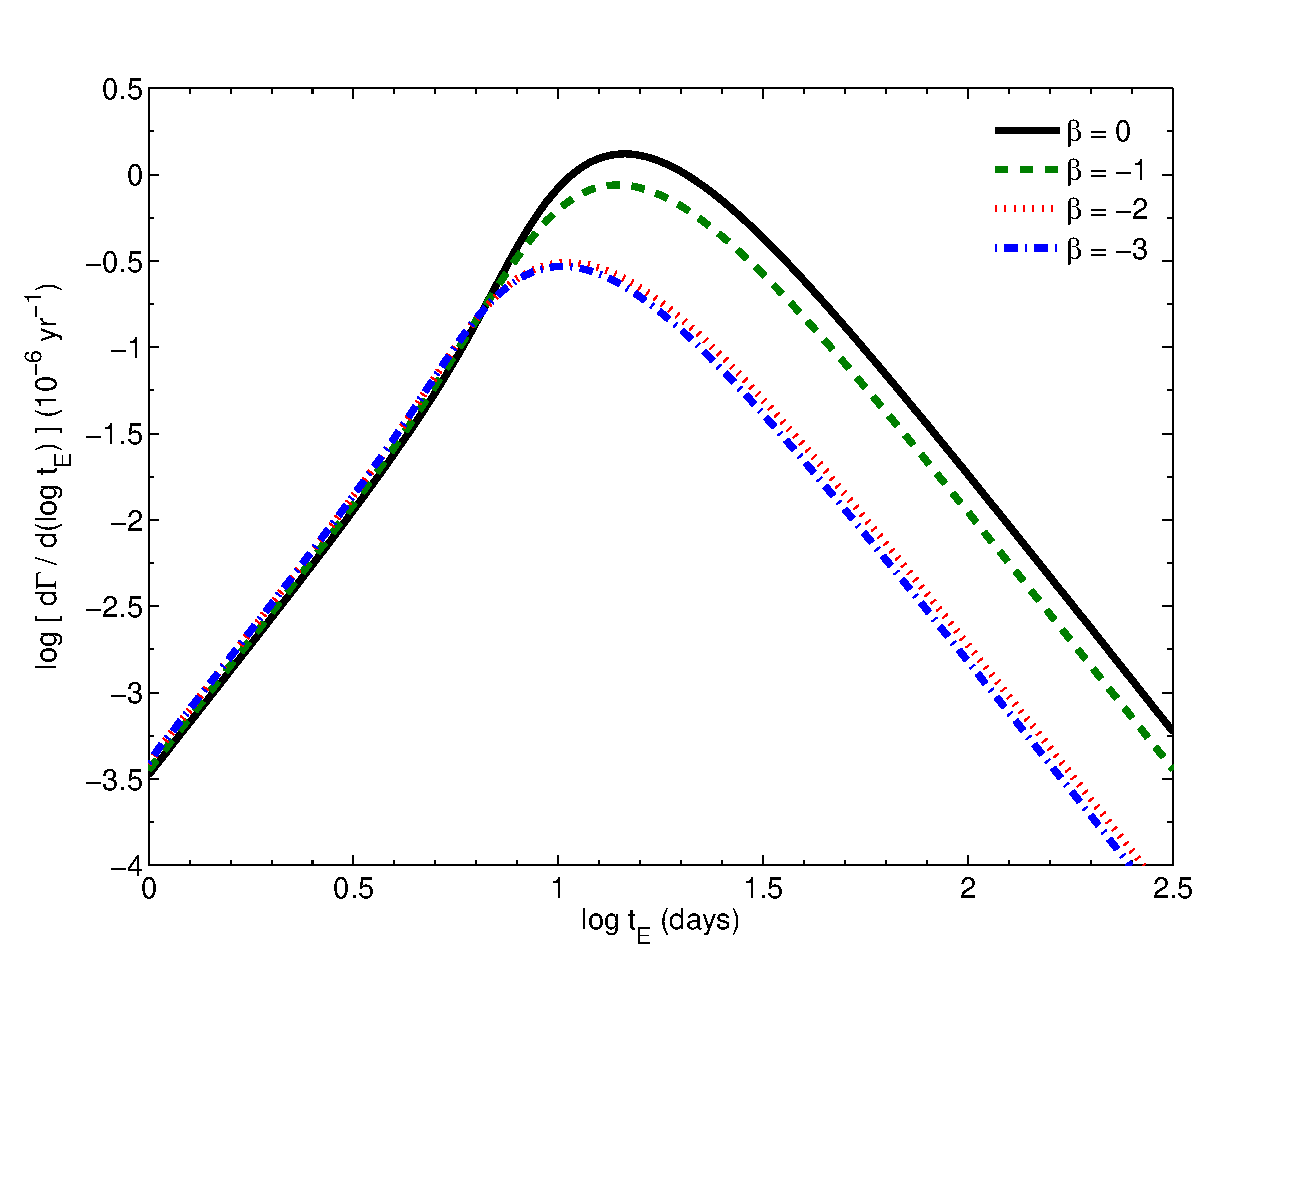
\includegraphics[width=4 in,trim=0 0 0 3cm]{time_beta.eps}
%
\caption{银心方向上中子星导致的微引力透镜事件的概率随时标的分布。实线、虚线、
点线和点虚线分别对应$\beta=0,-1,-2,-3$。}
\label{timescale_beta}
\end{center}
\end{figure}
%%%%%%%%%%%%%%%%%%%%%%%%%%%%%%%%%%%%%%%%%%
%

在WM05中,他们给出了在银心区域,平均的银河系微引力透镜事件(包含中子星
作为透镜天体以及其他天体作为透镜天体)的时标的等值图。我们计算得到的由中子
星导致的事件比较短的时标将降低平均的时标。在图\ref{map_timescale}中,
我们给出了银河系中心区域的微引力事件的平均时标的分布,可以与WM05中的
图3进行对比。实线代表$\beta=-1$的结果,彩色区域代表$\beta=-2$的结
果。OGLE-III的监测区域用菱形表示。在BW方向,取$\beta=0,-1,-2$,我们得到的
平均时标分别是23.3,23.9和36.5天。对于$\beta=0,-1$,我们的结果与WM05中
的结果接近,但是稍微小一些。我们的结果与OGLE观测的实际测量结果,$28.1\pm4.3$天\supercite{sumi},是符合的。

%%%%%%%%%%%%%%%%%%%%%%%%%%%%%%%%%%%%%%%%%
%
\begin{figure}
\begin{center}
  %
  \includegraphics[width=4 in,trim=0 0 0 3cm]{map_timescale.eps}
%
\caption{银河系微引力透镜事件平均时标的等值图。实线对应$\beta=-1$,
彩色区域对应$\beta=-2$。等值线代表以天为单位的平均时标。OGLE-III区域
用菱形表示。}
\label{map_timescale}
\end{center}
\end{figure}
%%%%%%%%%%%%%%%%%%%%%%%%%%%%%%%%%%%%%%%%%%
%

\subsubsection{中子星导致的事件占银河系总事件的比例}

我们结果已经显示了由中子星导致的微引力透镜事件的时标比较短。Sumi et al. (2011)\supercite{sumi11}
预计由木星质量的天体导致的微引力透镜事件有更短的时标,而由其他的天体
导致的事件的时标则要更长。在这一节中,我们考虑在不同的时标上,
由中子星导致的事件占银河系总事件的比例。

在图\ref{ratio}中,我们给出了由中子星导致的事件所占的比例随着时标
的分布。实线代表BW方向的事件,虚线代表银心方向的事件。我们也
给出了远离银心方向($(l,b)=(-20^{\circ},0^{\circ})$ 
和$(l,b)=(0^{\circ},-10^{\circ})$)的结果。对于$(l,b)=(-20^{\circ},0^{\circ})$
(在银盘上,但是远离银心方向)中子星作为透镜天体的贡献在时标
短于约10天时可以高达约40\%,但是我们强调在这个方向上总的
事件概率远比银心方向低。在另外的三个方向上,中子星导致的事件
所占比例均在约15天的时标上达到最大值,并且也是分布的极大值。
我们的结果与之前的工作给出的预计不同,WM05的结果在图\ref{ratio}中
用点虚线表示。他们的工作显示中子星作为透镜天体的事件将主要
在几百天的时标上占较大比例,而在15天左右的时标上所占比例很低。
我们的工作则预计,中子星导致的事件将主要贡献银河系中的较短
时标的微引力透镜事件,这是因为中子星有比较高的速度。在远离
银心的方向上,随着短时标的银河系微引力透镜事件数目的下降,
中子星导致的事件所占短时标事件的比例快速上升。

%
%%%%%%%%%%%%%%%%%%%%%%%%%%%%%%%%%%%%%%%%%
\begin{figure}
\begin{center}
  %
  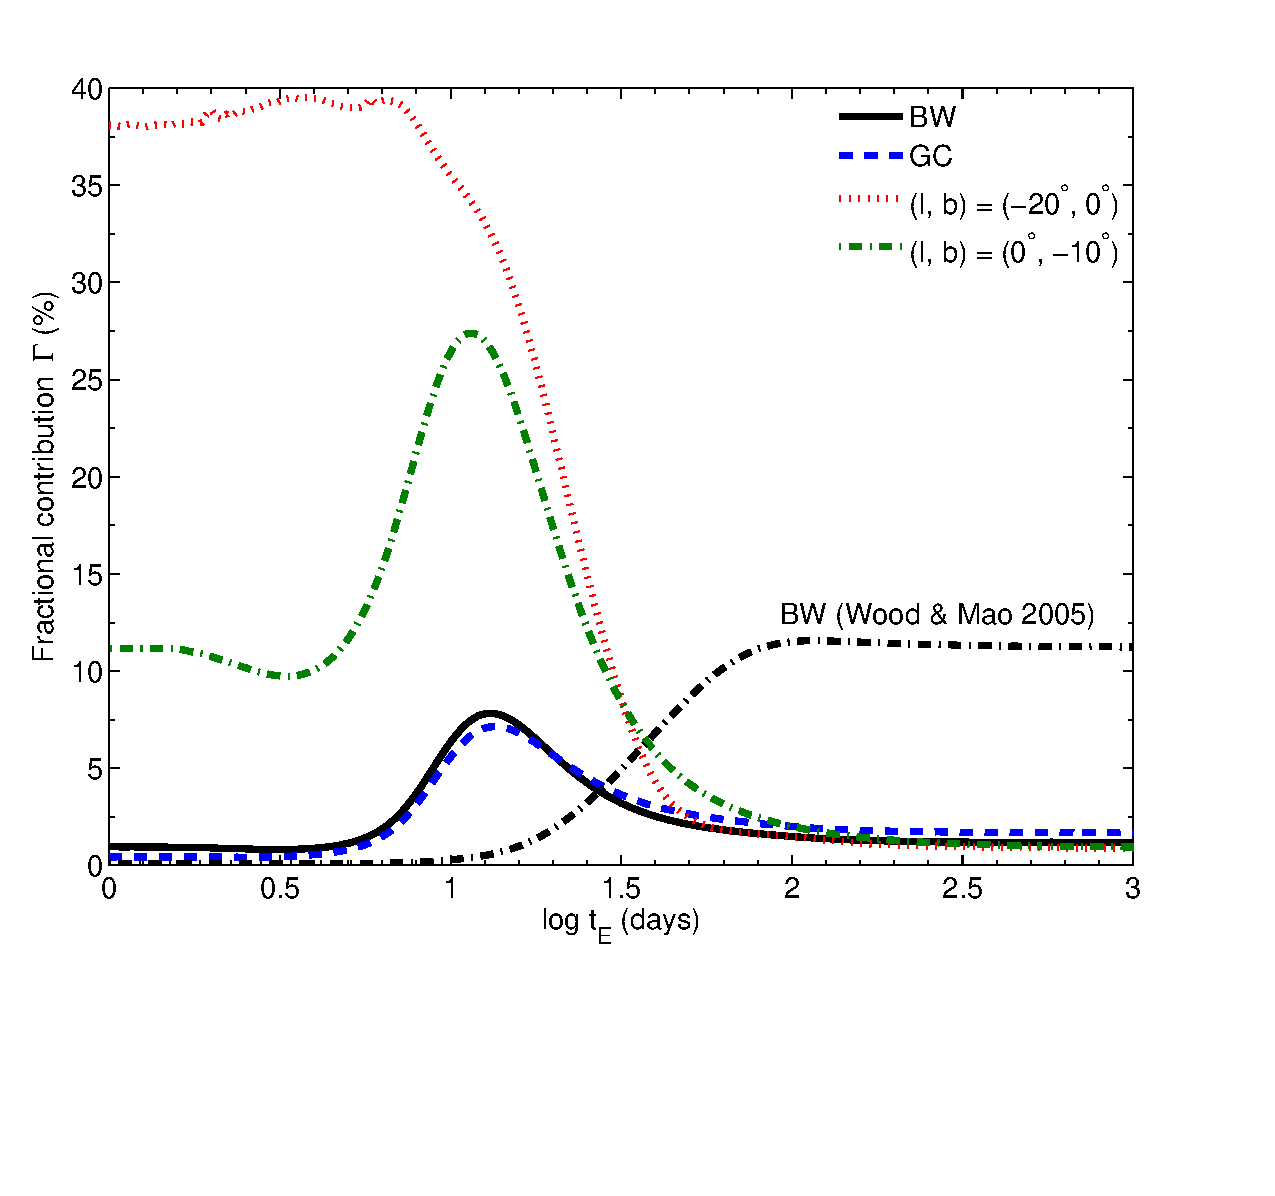
\includegraphics[width=4 in,trim=0 0 0 3cm]{ratio.eps}
%
\caption{中子星导致的微引力透镜事件占银河系总事件的比例随着事件时标的分布。
实线、虚线、点线和点虚线分别对应与BW、银心和远离银心方向($(l,b)=(-20^{\circ},0^{\circ})$
和$(l,b)=(0^{\circ},-10^{\circ})$)。作为对比,在BW方向上使用WM05的模型得到
结果也在图上画出。}
\label{ratio}
\end{center}
\end{figure}
%%%%%%%%%%%%%%%%%%%%%%%%%%%%%%%%%%%%%%%%%%
%

在图\ref{ratio_beta}中,我们给出了在银心方向上取不同的
$\beta$中子星作为透镜天体的贡献比。在所有情况下,贡献比都在
约10天的时标上达到最大值,并且都与WM05给出的结果不同。随着$\beta$的
减小,在10天左右的时标上由中子星导致的事件所占的比例升高。
对于$\beta=-3$,几乎所有的时标在10天左右的事件都是由中子星
导致的。
%
%%%%%%%%%%%%%%%%%%%%%%%%%%%%%%%%%%%%%%%%%
\begin{figure}
\begin{center}
  %
  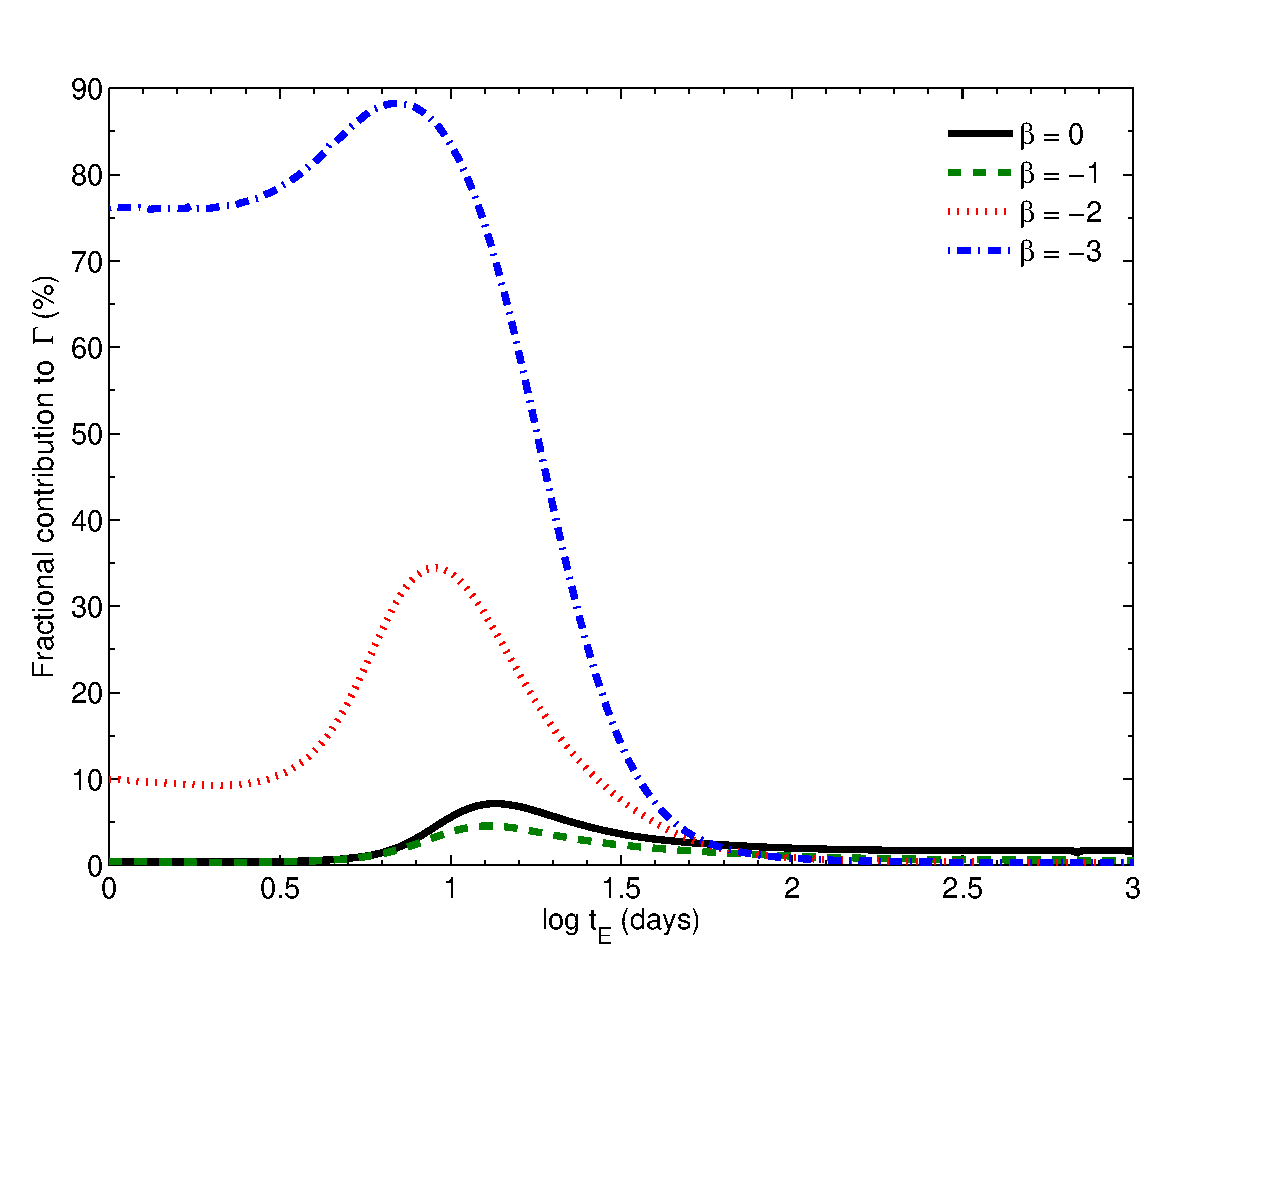
\includegraphics[width=4 in,trim=0 0 0 3cm]{ratio_beta.eps}
%
\caption{银心方向上,中子星导致的微引力透镜事件占银河系总事件的比例随着
事件时标的分布。实线、虚线、点线和点虚线分别对应$\beta=0,-1,-2,-3$。}
\label{ratio_beta}
\end{center}
\end{figure}
%%%%%%%%%%%%%%%%%%%%%%%%%%%%%%%%%%%%%%%%%%
%

中子星导致的事件占银河系总事件的比例在不同的方向上不同。在
图\ref{map_percentage}中,我们给出了中子星导致的事件所占比例
在银河系中心区域的等值图。实线对应$\beta=-1$,彩色区域对应
$\beta=-2$。OGLE-III的监测区域用菱形表示。中子星导致事件的比例
明显随着银经和银纬而变化,并且在远离银心区域所占比例比较高。
%
%%%%%%%%%%%%%%%%%%%%%%%%%%%%%%%%%%%%%%%%%
\begin{figure}
\begin{center}
  %
  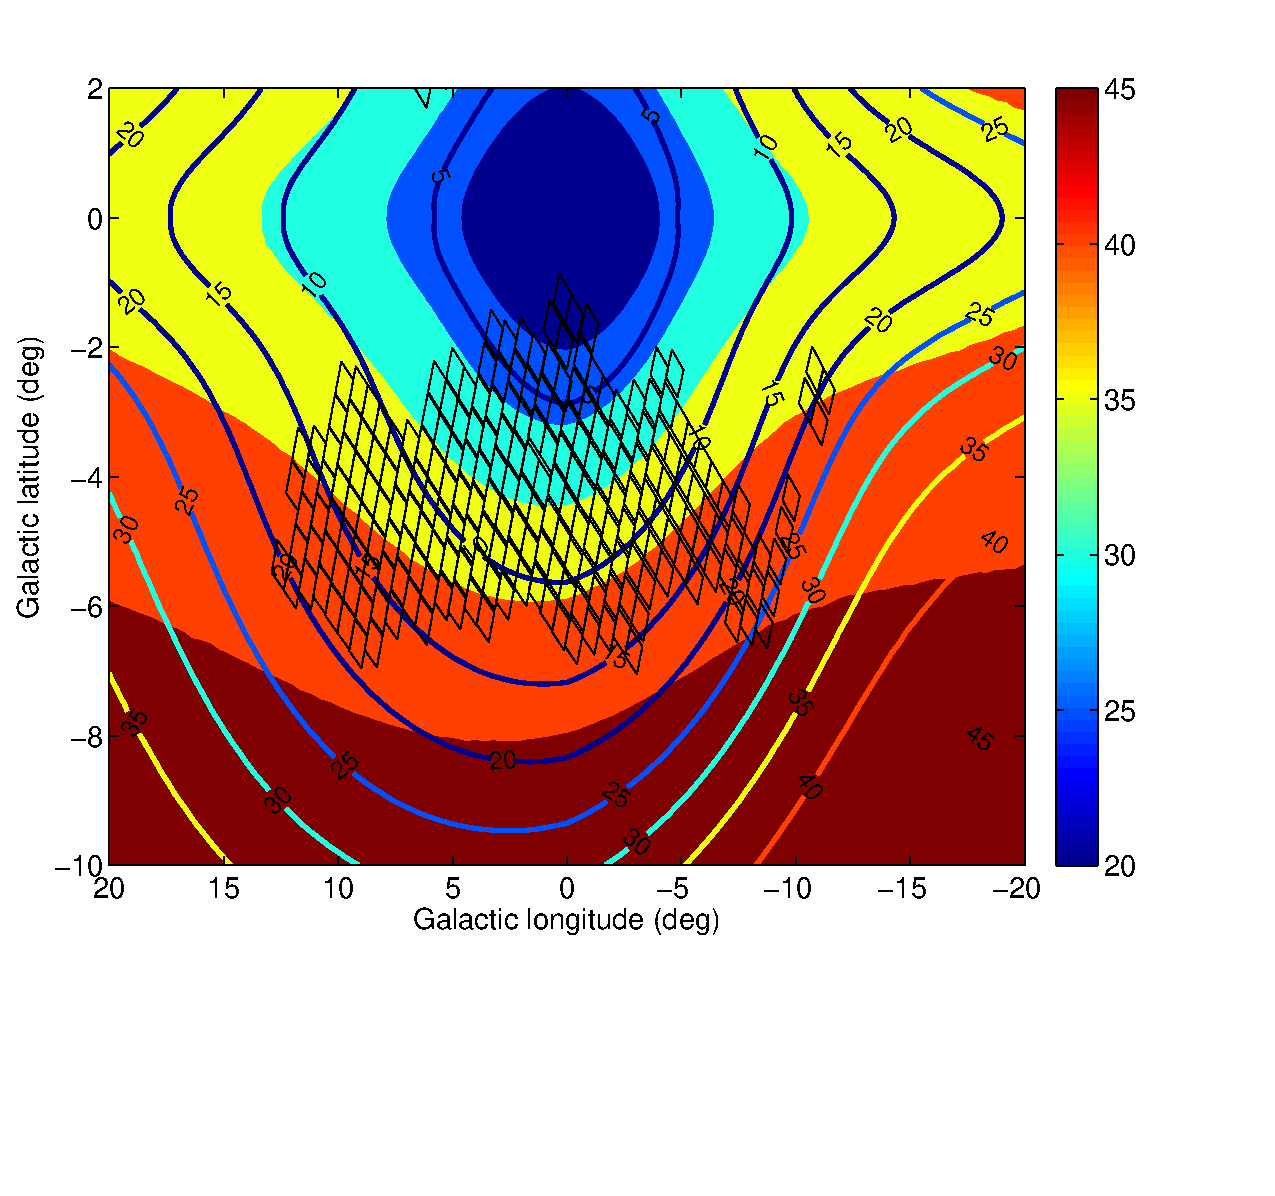
\includegraphics[width=4 in,trim=0 0 0 3cm]{map_percentage.eps}
%
\caption{中子星导致的微引力透镜事件占银河系总事件的比例的等值图。
实线对应$\beta=-1$,彩色区域对应$\beta=-2$。OGLE-III的监测区域用
菱形表示。}
\label{map_percentage}
\end{center}
\end{figure}
%%%%%%%%%%%%%%%%%%%%%%%%%%%%%%%%%%%%%%%%%%
%

在所有时标上进行平均,并且全天平均后,我们得到由中子星导致的微引力透镜
事件占银河系总事件的约5.4\%($\beta=0$)。在表\ref{percent}中,我们
给出了不同种类的天体作为透镜天体导致的事件占银河系总事件的比例。
我们的计算包含了褐矮星(BDs)、主序星(MSs)、白矮星(WDs)以及
黑洞(BHz)。我们也给出了对于不同的$\beta$值的结果。对于$\beta=0$,
中子星导致的事件所占比例比较低,然而随着$\beta$的下降,中子星导致事件
的贡献比例越来越高。通过增大和减小中子星速度分布的$\sigma$的30\%,
我们得到中子星导致的事件的贡献比分别为6.5\%和3.7\%($\beta=0$)。
使用指数的速度模型,我们得到的中子星导致事件的贡献比约是4.2\%($\beta=0$)。
%
%%%%%%%%%%%%%%%%%%%%%%%%%%%%%%%%%%%%%%%%%%%%%%%%%%%%%%%%%%%%%%%%%%%%%%%%%
\begin{table}
\begin{center}
\caption{不同种类的天体作为透镜天体对银河系总的事件概率的贡献比。
$\beta=-1,-2,-3$对应的结果被分别列出。作为对于,使用WM05模型得到
的结果也被列出。}
\label{percent}
%
\begin{tabular}{lccccc}
\hline
             &       \multicolumn{5}{c}{Types of lens}      \\
$\beta$      & BD   &    MS    &    WD     &  BH   & NS     \\
             &       \multicolumn{5}{c}{(per cent)}         \\
\hline
0            & 16.7 &    60.5  &    16.5   &  0.9  & 5.4    \\
-1           & 15.8 &    57.2  &    15.5   &  0.9  & 10.6   \\        
-2           & 10.6 &    38.2  &    10.4   &  0.5  & 40.3   \\         
-3           & 10.0 &    36.0  &    9.8    &  0.5  & 43.7   \\            
0 (WM05)     & 17.2 &    62.1  &    16.9   &  0.9  & 2.9    \\
\hline
\end{tabular}
\end{center}
\end{table}
%%%%%%%%%%%%%%%%%%%%%%%%%%%%%%%%%%%%%%%%%%%%%%%%%%%%%%%%%%%%%%%%%%%%%%%%%%
%
%

\subsection{通过astrometric microlensing测量脉冲星质量}

我们已经研究了由中子星导致的photometric microlensing事件的性质。
然而,由可观测射电脉冲星导致的photometric microlensing的事件概率
是比较低的,对于$10^{10}$颗背景天体,事件概率是约两个事件每十年。
由于astrometric microlensing事件发生的截面比photometric microlensing事
件大得多,更多的astrometric microlensing事件可能被探测到。目前
还没有可以预见的大规模的针对astrometric microlensing的巡天。于是
更可行的寻找由脉冲星导致的astrometric microlensing事件的方法是
使用已知的脉冲星的天体测量参数来预测引力透镜事件发生的时间和地点。
这个方法也可以用于搜寻由脉冲星导致的photometric microlensing事件,
但是astrometric microlensing更大的发生截面意味着更高的成功概率。

我们用于计算photometric microlensing的事件概率的方法可以直接被
用于astrometric microlensing事件概率的计算,只需要使用更大的
发生截面。Astrometric microlensing的发生截面和现象的强度可以
使用“impact parameter ($u_0$)”来刻画。$u_0$是透镜天体和背景天体
之间角距离的最小值,单位是Einstein半径。于是astrometric microlensing的
事件概率可以直接根据截面增大的倍数放大photometric microlensing的
事件概率来估算。比如,如果astrometric microlensing的截面
是photometric microlensing的10倍(意味着$u_0=10$,在后面的小节中
会进一步讨论这个取值),那么假设$\beta=-1$以及$10^{10}$
颗背景天体,对于120000颗可观测的射电脉冲星,全天平均的事件概率是$\sim1.5$每年,

\subsubsection{Astrometric microlensing模型}

Belokurov \& Evans (2002)\supercite{Bel}(缩写为BE02)给出了
确定通过astrometric microlensing现象测量透镜天体质量的精度的
方法。他们说明了对于常规天体作为透镜天体的情况,有11个参数
需要通过观测确定。在我们后面的计算中,我们使用了BE02给出的方法,
但是我们主要是讨论射电脉冲星作为透镜天体的情况。

对于射电脉冲星作为透镜天体的情况,透镜天体的位置、自行以及
距离可以独立地通过射电观测得到。脉冲星的位置和自行可以通过
射电脉冲星的测时或者射电干涉观测确定。对于有多年观测数据
的射电脉冲星,通过测时得到的位置和自行的精度可以分别达到
$\leq 1$\,mas和$\leq 1$\,$\rm{mas\ yr^{-1}}$\supercite{verbiest}。
对于那些不能通过高精度测时来得到位置和自行的脉冲星,射电
干涉观测可以用于精确测量这些参数\footnote{我们指出,脉冲星测时
使用的dynamical solar system ephemeris与International Celestial 
Reference Frame (ICRF)不同。Madison et al. (2013)\supercite{Madison13}
计算了ICRF与脉冲星测时坐标系统的转换,并且讨论了在未来这样的
转化能如何通过更多的观测改进。}。在我们的模型中我们考虑一种
理想情况,假设射电脉冲星的位置和自行都是已知的参数,并且忽略
他们的测量误差。脉冲星的位置和自行的测量误差对我们的计算的影响
会在最后进行讨论。

脉冲星的距离相比位置和自行要更难确定。一些脉冲星的距离可以通过
视差的测量精确给出。但是对于大部分脉冲星来说,距离只能通过
色散测量(dispersion measures)来估算。通过色散测量来估计脉冲星
的距离依赖于银河系的自由电子密度分布的模型,而这一模型目前还不成熟,
于是导致通过这一方法估算距离的误差达到20\%\supercite{Taylor}。
尽管人们一直在改进银河系自由电子密度模型\supercite{cordes},但是
还不清楚到我们发现由脉冲星导致的微引力透镜事件时脉冲星的距离能不能
通过色散测量精确确定。因此,在我们的模型中我们考虑了两种情形。
第一种情形,称作Model $D_{\rm{psr}}^{\rm{known}}$,我们假设脉冲星
的距离是已知的;第二种情形,称作Model $D_{\rm{psr}}^{\rm{unknown}}$,
我们假设脉冲星的距离是未已知的。

对于Model $D_{\rm{psr}}^{\rm{known}}$,我们有六个独立参数需要
通过引力透镜效应的观测来确定,分别是背景天体的位置($\bm{\theta_{\rm{s,0}}}$)、
自行($\bm{\mu_{\rm{s}}}$)和视差($\pi_{\rm{s}}$),以及透镜天体的质量($M$)。
我们指出,背景天体的天体测量参数有可能也是精确知道的。这种情况下
我们只需要确定透镜天体的质量这一个参数,而在我们的工作中我们假设
这些参数是未知的,需要通过引力透镜效应的观测确定。对于Model $D_{\rm{psr}}^{\rm{unknown}}$,
我们还需要测量脉冲星的视差($\pi_{\rm{l}}$),于是有七个独立参数
需要确定。

我们考虑使用PSR B1929$+$10这颗脉冲星作为一个例子来研究。这颗脉冲星
有很大的自行(103\,$\rm{mas\ yr^{-1}}$)\supercite{Chatterjee04},
并且投影位置与多颗光学天体很近。根据我们对比已知脉冲星的位置\supercite{Manchester05}\footnote{http://www.atnf.csiro.au/research/pulsar/psrcat} 
与UKIRT Infrared Deep Sky Surveyd(UKIDSS)的源表\supercite{Lawrence}
的结果,在这颗脉冲星位置周围5\,arcsecs的范围内有七颗光学天体。
这颗脉冲星的距离是0.36\,kpc\supercite{Chatterjee04}。我们假设
这颗脉冲星很可能很近地经过一颗背景天体,并且我们进行一个持续四年
的对背景天体的位置的精确监测。我们假设观测采样在四年之内是均匀的,
并且以astrometric microlensing效应最强时作为时间中点。我们同时
假设背景天体的距离是5\,kpc,自行是7\,$\rm{mas\ yr^{-1}}$。

%
我们强调我们选择的透镜天体和背景天体的自行和距离不会影响我们
的研究的普遍性,因为astrometric microlensing效应的幅度是由并且
只由$u_0$决定。然而,透镜天体质量测量的精度与几个参数的选取有关。
首先是脉冲星的质量。在我们的计算中,我们使用$M=1.4$\,$\rm{M_{\odot}}$作
为典型的脉冲星质量,但是我们也尝试了其他的质量并且进行讨论。
其次我们需要假设背景天体的位置测量的精度。我们使用了两个可能
的取值,$\sigma=150$和450\,$\rm{\mu as}$。$\sigma=150$\,$\rm{\mu as}$
对应于\textit{Gaia}卫星对于一颗比较亮的源($V=16$\,mag)能达到的精度
\footnote{我们使用了\url{http://www.cosmos.esa.int/web/gaia/science-performance} 
提供的信息来估算单次观测的视差测量精度。对于$V=16$\,mag的
一个天体,\textit{Gaia}最终能达到的视差测量精度是约20-40\,$\rm{\mu as}$。
单次测量的视差精度会比这个差,约是这个值的4.3倍。单次观测的位置
测量的精度比视差测量的精度高,约是视差测量精度的0.743倍。于是我们
得到单次位置测量的精度大概是最终视差测量精度的三倍,约60-120\,$\rm{\mu as}$。
我们还需要考虑到\textit{Gaia}的单次观测只测量沿着扫描方向的一维的
位置,于是二维位置测量的精度需要乘以$\sqrt{2}$。考虑了以上因素之后
我们得到对于$V=16$\,mag的一个天体,单次二维位置测量的精度约是90-120\,$\rm{\mu as}$。
而对于更暗的天体($V=20$\,mag),\textit{Gaia}最终达到的视差测量
精度降到130-600\,$\rm{\mu as}$,这意味着单次二维位置测量的精度
只有0.5-3\,mas。}。未来的望远镜,比如Wide-Field Infrared Survey 
Telescope(WFIRST),即使对更暗的天体也能达到几十分之一毫角秒
的位置测量精度\supercite{Spergel}。最后我们还需要假设我们在整个
四年的监测中的观测频率,即总的观测数目。在我们的计算中我们尝试
了不同的观测频率,并进行了讨论。

\subsubsection{脉冲星质量测量}


图\ref{mass_u0}展示了脉冲星质量测量的误差随着$u_0$的变化。
脉冲星距离已知和未知的两种情形的结果都分别给出。我们使用
了两组不同的采样数,15和100次观测。我们的结果显示,质量测量
的误差在不同情形下变化很大。随着$u_0$的增大,质量测量的误差增大,
而随着采样数的增大,质量测量的误差减小。如果脉冲星的距离已知,
脉冲星的质量测量的误差只有距离未知情形的一半。我们指出,对于\textit{Gaia}卫星采样数大概是70\supercite{DeBruijne12}。
%
%%%%%%%%%%%%%%%%%%%%%%%%%%%%%%%%%%%%%%%%%
\begin{figure}
\begin{center}
  %
  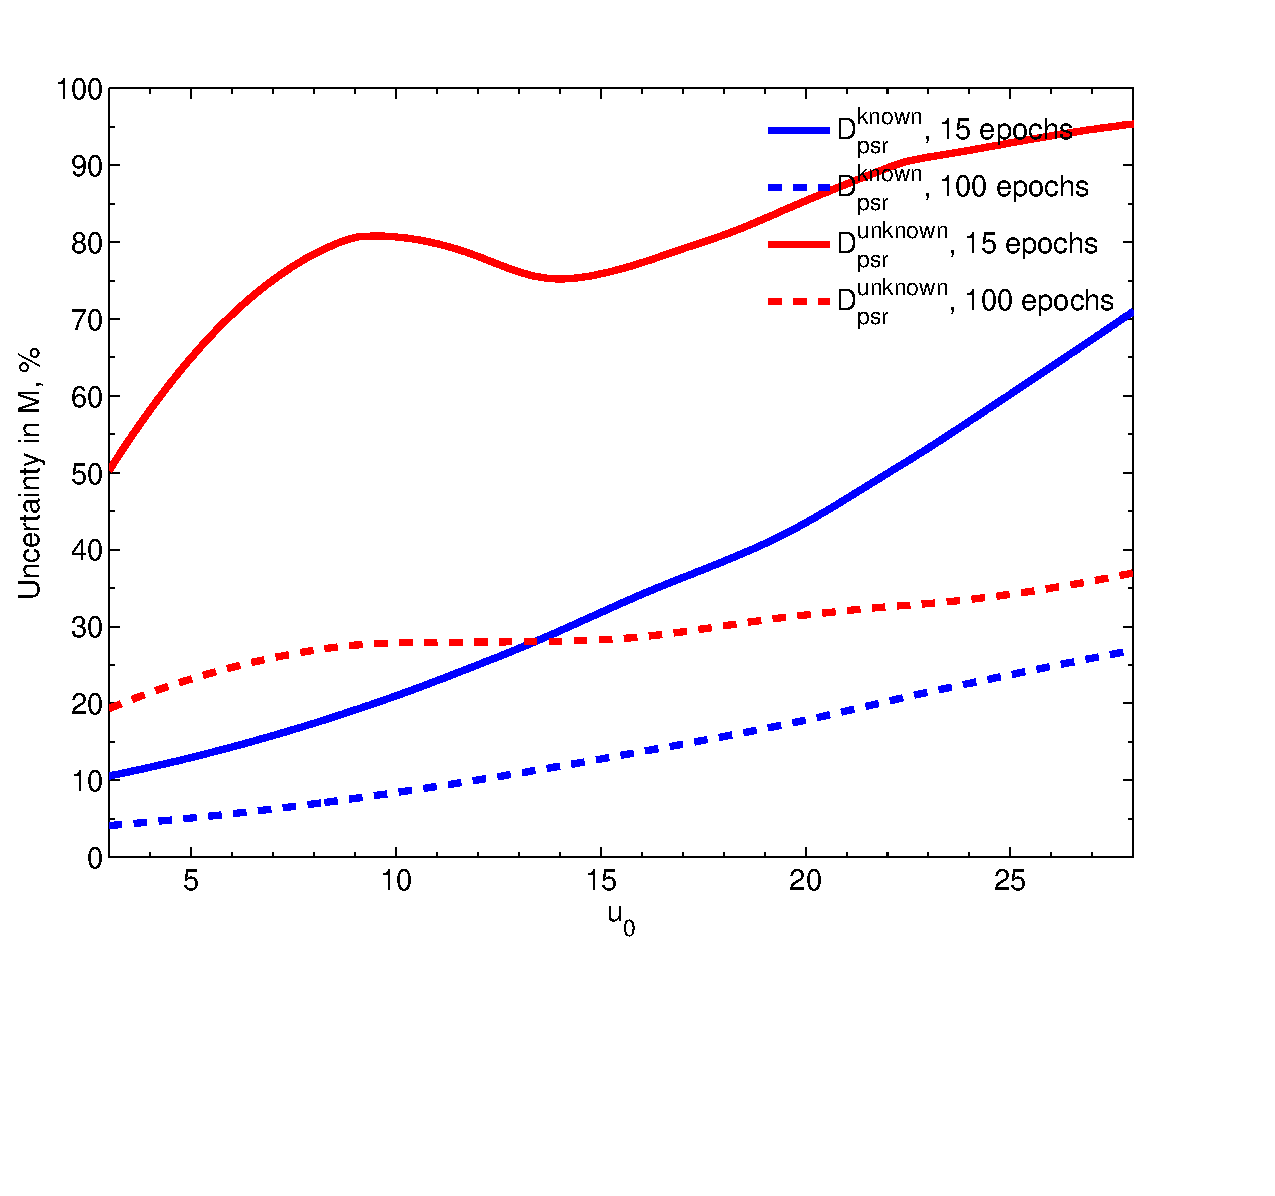
\includegraphics[width=4 in,trim=0 0 0 3.2cm]{u0_mass.eps}
%
\caption{质量测量的误差随着$u_0$的变化。误差是以
脉冲星质量为单位的。我们假设$M=1.4$\,$M_{\odot}$以及$\sigma=150$\,$\rm{\mu as}$。
实线和虚线分别代表采样数为$15$和$100$。红色和蓝色分别对应脉冲星距离
已知(Model $D_{\rm{psr}}^{\rm{known}}$)和未知(Model $D_{\rm{psr}}^{\rm{unknown}}$)的情形。
}
\label{mass_u0}
\end{center}
\end{figure}
%%%%%%%%%%%%%%%%%%%%%%%%%%%%%%%%%%%%%%%%%%

图\ref{mass_6}和\ref{mass_7}给出了质量测量的误差随观测的数目的变化。
在图\ref{mass_6}中,我们假设脉冲星距离是已知的,而在图\ref{mass_7}中
我们假设脉冲星距离是未知的。在两张图中,我们都给出了$u_0=10$和$u_0=30$,
以及$\sigma=150$\,$\rm{\mu as}$和$\sigma=450$\,$\rm{\mu as}$的四组结果。
我们发现,当观测数目大于$\sim$100时,质量测量的误差便几乎不再变化,
这说明更高的监测频率不是必须的,不会提高质量测量的精度。当背景天体
的位置测量精度从450\,$\rm{\mu as}$提高到150\,$\rm{\mu as}$,透镜
天体的质量测量精度提高了两倍。因此,为了精确地确定脉冲星的质量,
我们需要高精度的背景天体的位置测量。

%
%%%%%%%%%%%%%%%%%%%%%%%%%%%%%%%%%%%%%%%%%
\begin{figure}
\begin{center}
  %
  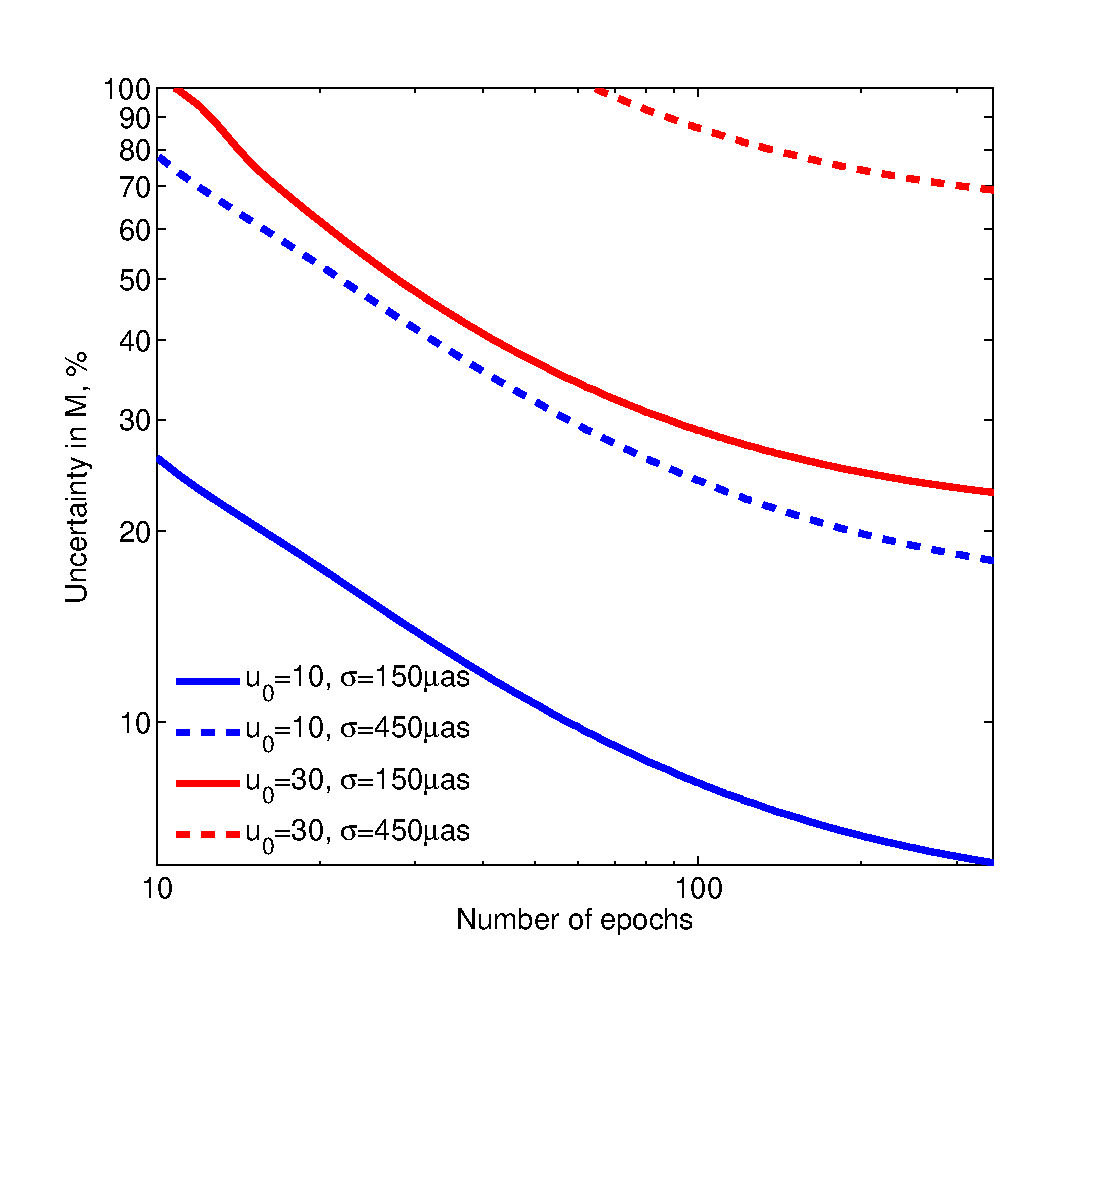
\includegraphics[width=4 in,trim=0 0 0 3.2cm]{mass_6.eps}
%
\caption{质量测量的误差随着观测数目的变化。误差是以
脉冲星质量为单位的。我们假设$M=1.4$\,$M_{\odot}$,并且假设
脉冲星的距离已知(Model $D_{\rm{psr}}^{\rm{known}}$)。
我们给出了对应不同的$u_0$和$\sigma$的结果。
}
\label{mass_6}
\end{center}
\end{figure}
%%%%%%%%%%%%%%%%%%%%%%%%%%%%%%%%%%%%%%%%%%
%
%
%%%%%%%%%%%%%%%%%%%%%%%%%%%%%%%%%%%%%%%%%
\begin{figure}
\begin{center}
  %
  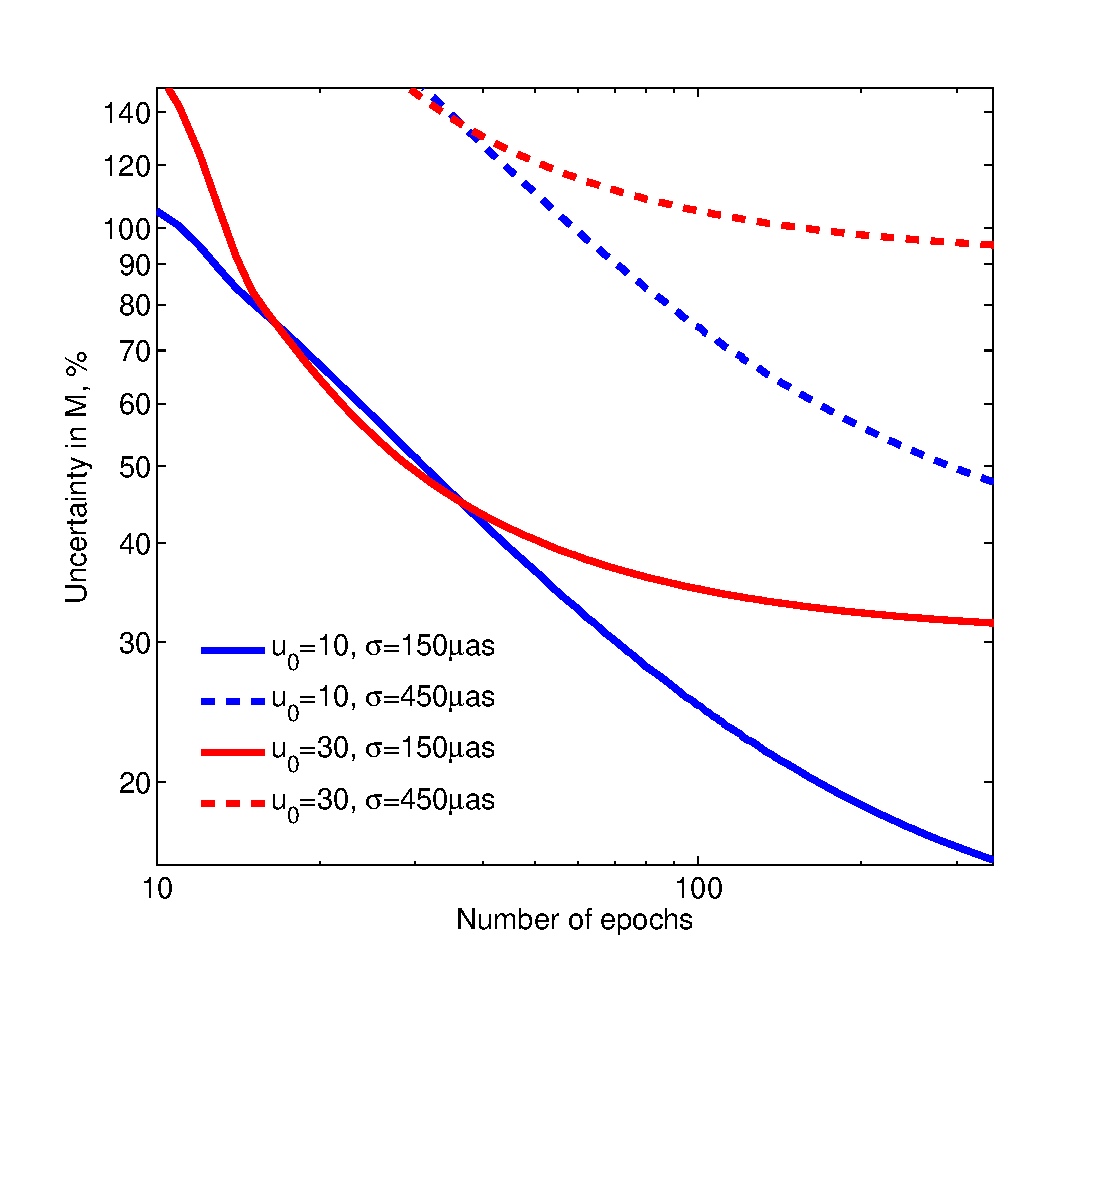
\includegraphics[width=4 in,trim=0 0 0 3.2cm]{mass_7.eps}
%
\caption{质量测量的误差随着观测数目的变化。误差是以
脉冲星质量为单位的。我们假设$M=1.4$\,$M_{\odot}$,并且假设
脉冲星的距离未知(Model $D_{\rm{psr}}^{\rm{unknown}}$)。
我们给出了对应不同的$u_0$和$\sigma$的结果。
}
\label{mass_7}
\end{center}
\end{figure}
%%%%%%%%%%%%%%%%%%%%%%%%%%%%%%%%%%%%%%%%%%
%

在图\ref{masses}中,我们假设了不同的脉冲星质量,并且假设脉冲星
距离已知(Model $D_{\rm{psr}}^{\rm{known}}$),然后给出了质量
测量的误差随着观测数目的变化。我们假设$u_0=10$以及$\sigma=450$\,$\rm{\mu as}$。
除了典型的脉冲星质量,1.4\,$\rm{M_{\odot}}$,我们还使用了极低的
脉冲星质量,0.4\,$\rm{M_{\odot}}$,和极大的脉冲星质量,2.4\,$\rm{M_{\odot}}$。
我们发现,随着脉冲星质量的增大,质量测量的误差减小。对于大质量
脉冲星的情形(2.4\,$\rm{M_{\odot}}$),质量测量的误差比小质量脉
冲星的情形(0.4\,$\rm{M_{\odot}}$)小六倍。
%
%%%%%%%%%%%%%%%%%%%%%%%%%%%%%%%%%%%%%%%%%
\begin{figure}
\begin{center}
  %
  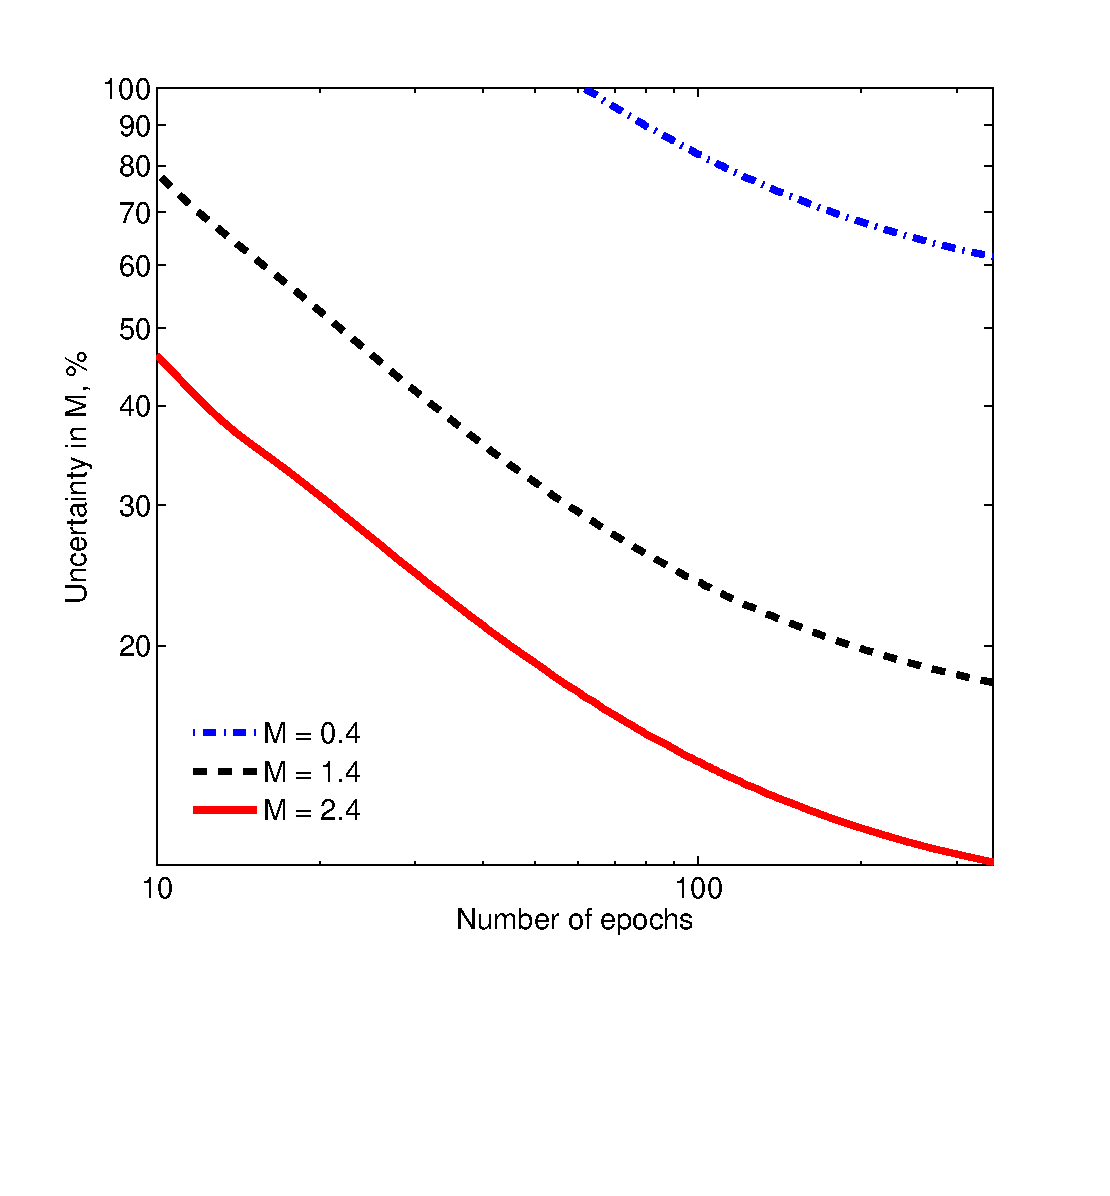
\includegraphics[width=3.5 in,trim=0 0 0 3.2cm]{masses.eps}
%
\caption{质量测量的误差随着观测数目的变化。误差是以脉冲星质量为
单位的。我们分别取$M=0.4,1.4,2.4$\,$M_{\odot}$。
我们假设脉冲星距离已知(Model $D_{\rm{psr}}^{\rm{known}}$)。
}
\label{masses}
\end{center}
\end{figure}
%%%%%%%%%%%%%%%%%%%%%%%%%%%%%%%%%%%%%%%%%%
%

在以上的计算中,我们假设了一种理想情况,即脉冲星的位置和自行可以被精确地
测量并且测量误差可以被忽略不计。如果脉冲星的天体测量参数不能被独立地测量,
那么我们将需要通过引力透镜效应的观测来确定它们,从而将降低我们测量
透镜天体质量的精度。现在我们讨论一种中间情形,脉冲星的位置和自行可以
被独立地测量,但是测量误差不能被忽略。我们将这些参数的误差模拟为背景天体
位置测量的误差,然后使用相同的方法来研究透镜天体质量测量的精度。我们
假设脉冲星位置和自行测量的误差分别为0.01\,$\rm{mas}$和0.1\,$\rm{mas\ yr^{-1}}$。
这是目前通过Very Long Baseline Interferometry(VLBI)可以达到的精度\supercite{deller}。
假设脉冲星距离已知(Model $D_{\rm{psr}}^{\rm{known}}$)以及$u_0=10$和50次
观测,我们发现脉冲星质量的误差从约10\%增加到12\%。对于更大的脉冲星
位置和自行的误差,0.1\,$\rm{mas}$和1\,$\rm{mas\ yr^{-1}}$,质量测量的
误差约为22\%。因此我们得出结论,脉冲星的位置和自行的误差将引入额外
的质量测量误差,但是影响比较小,而且通过提高脉冲星位置和自行
的测量精度可以降低这一影响。

\subsection{小结}

有多个测光的大型巡天正在或者即将在不远的将来开始,这些巡天项目将主要
集中在银河系中心和银盘上,比如OGLE-IV、Vista Variable in the Via Lactea~\supercite{Minniti} 
和WFIRST~\supercite{Spergel}。在不远的将来LSST\supercite{ivez}将每三天
监测10000平方度的天区两次。
这样的巡天预计将对$r\sim24.5$ (AB)的点源达到$5\sigma$的深度的观测。
目前还不清楚LSST是否会搜寻银盘和银核,即使不会大范围地监测银盘和银核,
LSST也将监测$10^{10}$量级的银河系天体;而如果包含银盘和银核,监测
的银河系天体的数目将更大。另外,一个三年的HST项目计划发现在银河系中心
方向的由银河系内的黑洞和中子星导致的微引力透镜事件\supercite{sahu}。

我们的计算表明:
\begin{itemize}
\item 由中子星导致的微引力透镜事件的时标比之间预计的短,只有约20天左右。
\item 在银河系中心方向,在时标为15天左右的事件中,有大约7\%是由中子星
导致的。而在远离银心方向,对于时标短于20天的事件,由中子星导致的事件
所占的比例将高达40\%。
\item 通过astrometric microlensing效应,如果脉冲星的距离已知,脉冲星的
质量测量的精度可以达到约10\%。通过足够多的观测次数,即使脉冲星的距离
未知,脉冲星的质量也可以测量精确到25\%。
\end{itemize}

对于正在进行中的巡天,我们建议:
\begin{itemize}
\item 为了能尽可能多的探测到由中子星导致的微引力透镜事件,巡天应该
集中在银盘和银河系中心区域。
\item 为了发现由中子星导致的微引力透镜事件,我们应该集中搜寻短时标的
微引力透镜事件,并使用射电望远镜定点观测这些候选体以发现射电脉冲星。
\item 当新的射电脉冲星被发现后,他们的天体测量参数应该被精确的测量,
并且与已知的光学巡天结果进行对比。如果发现脉冲星有可能经过背景天体,
引发astrometric microlensing效应,那么我们可以预测事件发生的时间并
使用光学望远镜监测这个背景天体。
\item 尽管通过射电脉冲星的参数预测微引力透镜事件并使用光学望远镜
定点观测是最佳的策略,但是像\textit{Gaia}卫星这样的项目也不可忽
视。\textit{Gaia}总共将观测$10^9$颗银河系天体,根据我们的估算,在整个
项目期间(五年)将发现一个由可观测射电脉冲星导致的事件。
\end{itemize}

在更远的将来,大型射电望远镜将发现大部分银河系内可观测的射电脉冲星。
因此我们很可能发现由可观测的射电脉冲星导致的微引力透镜事件,并以此
测量脉冲星的质量。这样的测量将促进我们对中子星的理解,并且揭示
中子星的内部结构和致密物质的物态。

\pkuthssffaq

